\section{Experimental Detail} \label{sec:exp_details}


\subsection{Environment}
We implemented our Attention kernels using OpenAI Triton~\citep{openaitriton} and conducted experiments on Ubuntu 22.04 servers. Tests on the RTX 4090 utilized a server with PCIE 5.0, a 16-core Xeon(R) 6430 CPU, and 120GB DDR4 RAM, while the RTX3090 tests employed a server with a 16-core Xeon(R) 8358P CPU and 80GB DDR4 RAM.
To reproduce our results, experiments should be conducted in the environment of torch 2.4.0+cu121, triton-nightly (version of 20240816), python 3.11, and (gcc, g++) in version 9.

\subsection{Hyper-parameters for Attention Kernels}

We use 128 for a block size of $Q$, and 64 for a block size of $K$ and $V$.
The parameters {Num\_Warps} and {Num\_Stages}, which represent the number of warp schedulers and the number of processing stages in our GPU kernels, respectively, are detailed in Table~\ref{tab:kernel_para}.



\begin{table}[!htb]
\caption{Hyper-parameters for our Attention Kernels.}
\label{tab:kernel_para}
\setlength\tabcolsep{12pt}
\centering 
    \begin{tabular}{c|c|c|c} 
    \toprule
    \textbf{HeadDim} & \textbf{Causal Mask} & \textbf{Num\_Warps} & \textbf{Num\_Stages} \\
    \hline
    \bf 64  & \bf False & 4 & 3 \\ 
    \bf 64  & \bf True  & 4 & 4 \\
    \bf 128 & \bf False & 8 & 3 \\
    \bf 128 & \bf True  & 8 & 5 \\  \bottomrule
    \end{tabular}
\end{table}


\subsection{Details of datasets and models}
We choose the first 256 annotations from the COCO 2014val dataset as the prompt set for \ultrapixel and \unidiffuser image generation.
We also used the corresponding 256 images of the 256 prompts as the ground truth images to calculate the FID and sFID.
For \cogvideo, the model is trained on long texts, so we applied an open-sora prompt set, each consisting of more than 120 words.
The specific model we used for \timm is \textit{vit\_base\_patch16\_224.augreg2\_in21k\_ft\_in1k}.


\subsection{Additional Experiments} \label{sec:append_add_exp}


\begin{table}[h!]
\caption{Comparison of SageAttention with AWQ (W4A16) on Llama2.}
\label{tab:comp_awq}
\setlength\tabcolsep{2pt}
\centering
\begin{tabular}{l|c|c|c|c}
\toprule
 & Full-Precision & SageAttention & AWQ & AWQ+SageAttention \\
\hline
\textbf{Perplexity}$\downarrow$ & 5.4721 & \textbf{5.4729} & 5.5988 & 5.5998 \\
\textbf{Speedup of Linear Computation} & 0 & 0 & 0 & 0 \\
\textbf{Speedup of Attention} & 0 & \textbf{2x} & 0 & \textbf{2x} \\
\bottomrule
\end{tabular}
\end{table}

\begin{table}[h!]
\caption{Comparison of SageAttention with Q-diffusion (W8A8) on Unidiffuser.}
\label{tab:comp_qdiffusion}
\setlength\tabcolsep{15pt}
\centering
\begin{tabular}{l|c|c|c|c}
\toprule
 & FID$\downarrow$ & sFID$\downarrow$ & CLIP$\uparrow$ & ImageReward$\uparrow$ \\
\hline
\textbf{Full Precision} & 163.33 & 145.08 & 31.52 & 0.1609 \\
\textbf{SageAttention} & \textbf{166.49} & \textbf{143.18} & \textbf{31.54} & \textbf{0.1521} \\
\textbf{Q-diffusion (W8A8)} & 395.99 & 178.56 & 18.03 & -2.273 \\
\bottomrule
\end{tabular}
\end{table}

\begin{table}[h!]
\caption{Comparison of SageAttention with VIDIT-Q on CogvideoX.}
\label{tab:comp_viditq}
\setlength\tabcolsep{1.2pt}
\centering
\begin{tabular}{l|c|c|c|c|c|c}
\toprule
 & CLIPSIM$\uparrow$ & CLIP-T$\uparrow$ & VQA-a$\uparrow$ & VQA-t$\uparrow$ & FScore$\uparrow$ & End-to-end Speedup$\uparrow$ \\
\hline
\textbf{Full Precision} & 0.1837 & 0.9976 & 68.962 & 75.925 & 3.7684 & - \\
\textbf{SageAttention} & 0.1836 & 0.9976 & 68.839 & \textbf{75.037} & 3.8339 & \textbf{34.3\%} \\
\textbf{VIDIT-Q (W8A8)} & 0.1884 & 0.9974 & 68.185 & 71.011 & 3.7342 & 22\% (theoretical maximum) \\
\bottomrule
\end{tabular}
\end{table}


\subsection{Comparison with other methods}

There are some task-specific quantization methods, such as AWQ for LLMs, Q-diffusion for text-to-image, and ViDiT-Q for text-to-video applications. 
SageAttention is orthogonal to them because those works are mainly used to quantize the linear layers. Second, AWQ is only used to compress the parameters of LLMs with no acceleration effect in computation. Q-diffusion has not reported its acceleration effect in their paper and provided codes with acceleration effect in its official repository. ViDiT-Q has not provided the codes with acceleration effect in its official repository. Nonetheless, we compare SageAttention with those works as follows.
(1) We compare the perplexity of Llama2-7B on WikiText and the speedup in the prefilling stage. The results are shown in Table~\ref{tab:comp_awq}.
We compare SageAttention with Q-diffusion (W8A8) on Unidiffuser. The results are shown in Table~\ref{tab:comp_qdiffusion}.
We compare SageAttention with VIDIT-Q on CogvideoX and the results are shown in Table~\ref{tab:comp_viditq}. Since the official repository does not provide acceleration code, we estimate a theoretical maximum: the Linear layer accounts for 24\% of Cogvideo's latency, and W8A8 offers \textbf{at most} 4x speedup for the Linear layer, resulting in a theoretical maximum end-to-end speedup of $\frac{100}{100 - 24 \times \frac{3}{4}}\% = 22\%$.




\subsection{Some Insights}
Table~\ref{tab:quant_type_analysis} shows that the metric of Llama2 remains stable with quantization. The reason is that the distribution of $Q, K$, and $V$ in the attention of Llama2-7B is relatively uniform. As a result, quantizing $Q, K$, and $V$ to INT8 or FP8 does not significantly impact the accuracy of attention. This insight inspires the idea that better control over outlier activations in models could lead to more precise quantization results.
As works like \citet{fu2024moa,zhang2024sageattention2,zhang2025sageattention2_wksp}, we believe \our can also be effectively applied to various applications related to Transformers, such as MOE systems~\citep{wang2024remoe}, linear layer quantization~\citep{hu2025quant,zhang2025int8train,zhao2024vidit}, RAG systems~\citep{sagerag}, training optimization~\citep{li2023memory,li2025optimization,huang2024pruninglargelanguagemodels,xi2024coat}, heterogeneous GPU systems~\citep{jiang2025demystifying,jianghexgen,jianghexgen2}, and diffusion models acceleration~\citep{zheng2024masked,zheng2024diffusion,zheng2025elucidating,fu2024framefusion,zhao2024mixdq,xi2025sparse,zhang2025spargeattn,zhang2025spargeattn_wksp,yang2025sparse,zhang2025sageattention3,zhang2025sageattention2++}.


\begin{table}[!htb]
\caption{SageAttention based on Torch Attention.}
\label{tab:torch+sage}
\setlength\tabcolsep{12pt}
\centering 
    \begin{tabular}{c|c|c} 
    \toprule
    \textbf{Sequence Length} & \textbf{Torch Attention} & \textbf{SageAttention based on Torch Attention} \\
    \hline
    \bf 1024  & 46 & 48 \\ 
    \bf 2048  & 42  & \textbf{55} \\
    \bf 4096 & 55 & \textbf{87} \\
    \bf 8192 & OOM  & OOM \\  \bottomrule
    \end{tabular}
\end{table}

\section{Implementation based on Torch Attention}
FlashAttention is the state-of-the-art and most commonly used standard attention; another commonly used attention is Torch attention~\citep{pytorchBackend2024}. We report the implementation speeds based on Torch in Table~\ref{tab:torch+sage}.









\begin{table}[htb!]
    \centering
    \caption{Numerical error of $Q \cdot K$ using different type of quantization.}
    \label{tab:qk_error}
    \setlength\tabcolsep{12pt}
    \begin{tabular}{c||c|c}
        \toprule
        {\bf Data Type}  & {\bf Cosine Sim}  & {\bf Relative L1}   \\ \hline
        \bf INT8   &   \textbf{99.54\%}    & \textbf{0.084}   \\ 
        E4M3   &   92.83\%    & 0.342   \\ 
        E5M2   &   77.95\%    & 0.681   \\ \bottomrule
    \end{tabular}
\end{table}

\begin{table}[htb!]
    \caption{Error of quantized attention with or without smoothed K.}
    \begin{center}
    \label{tab:append_smooth_k}
    \begin{tabular}{c|c||c|c|c}
    \toprule
    {\bf Quantization Type}  & {\bf Smoothed K}  & {\bf Cosine Sim $\uparrow$}  & {\bf Relative L1 $\downarrow$}  & {\bf RMSE $\downarrow$}
    \\ \hline
    \multirow{2}{*}{Per-token (\ourt)}   & Without   & 62.24\%  & 1.187  & 0.294 \\ % \cline{2-5}
    & \textbf{With}      & \textbf{99.47\%}  & \textbf{0.045}   & \textbf{0.031} \\ \hline
    \multirow{2}{*}{Per-block (\ourb)}   & Without   & 30.60\%  & 1.286  & 0.464 \\ % \cline{2-5}
    & \textbf{With}      & \textbf{99.31\%}  & \textbf{0.072}  & \textbf{0.035} \\ \hline
    \multirow{2}{*}{Per-tensor}  & Without   & 41.40\%  & 1.554  & 0.399 \\ % \cline{2-5}
    & \textbf{With}      & \textbf{98.06\%}  & \textbf{0.126}  & \textbf{0.059} \\ \hline
    \multicolumn{2}{c||}{FlashAttention-3 (quantized version)}  &  \textbf{26.76\%}   &  \textbf{2.5354}  &  0.5378 \\ \bottomrule
    \end{tabular}
    \end{center}
\end{table}



\begin{figure}[!htb]
    \centering
    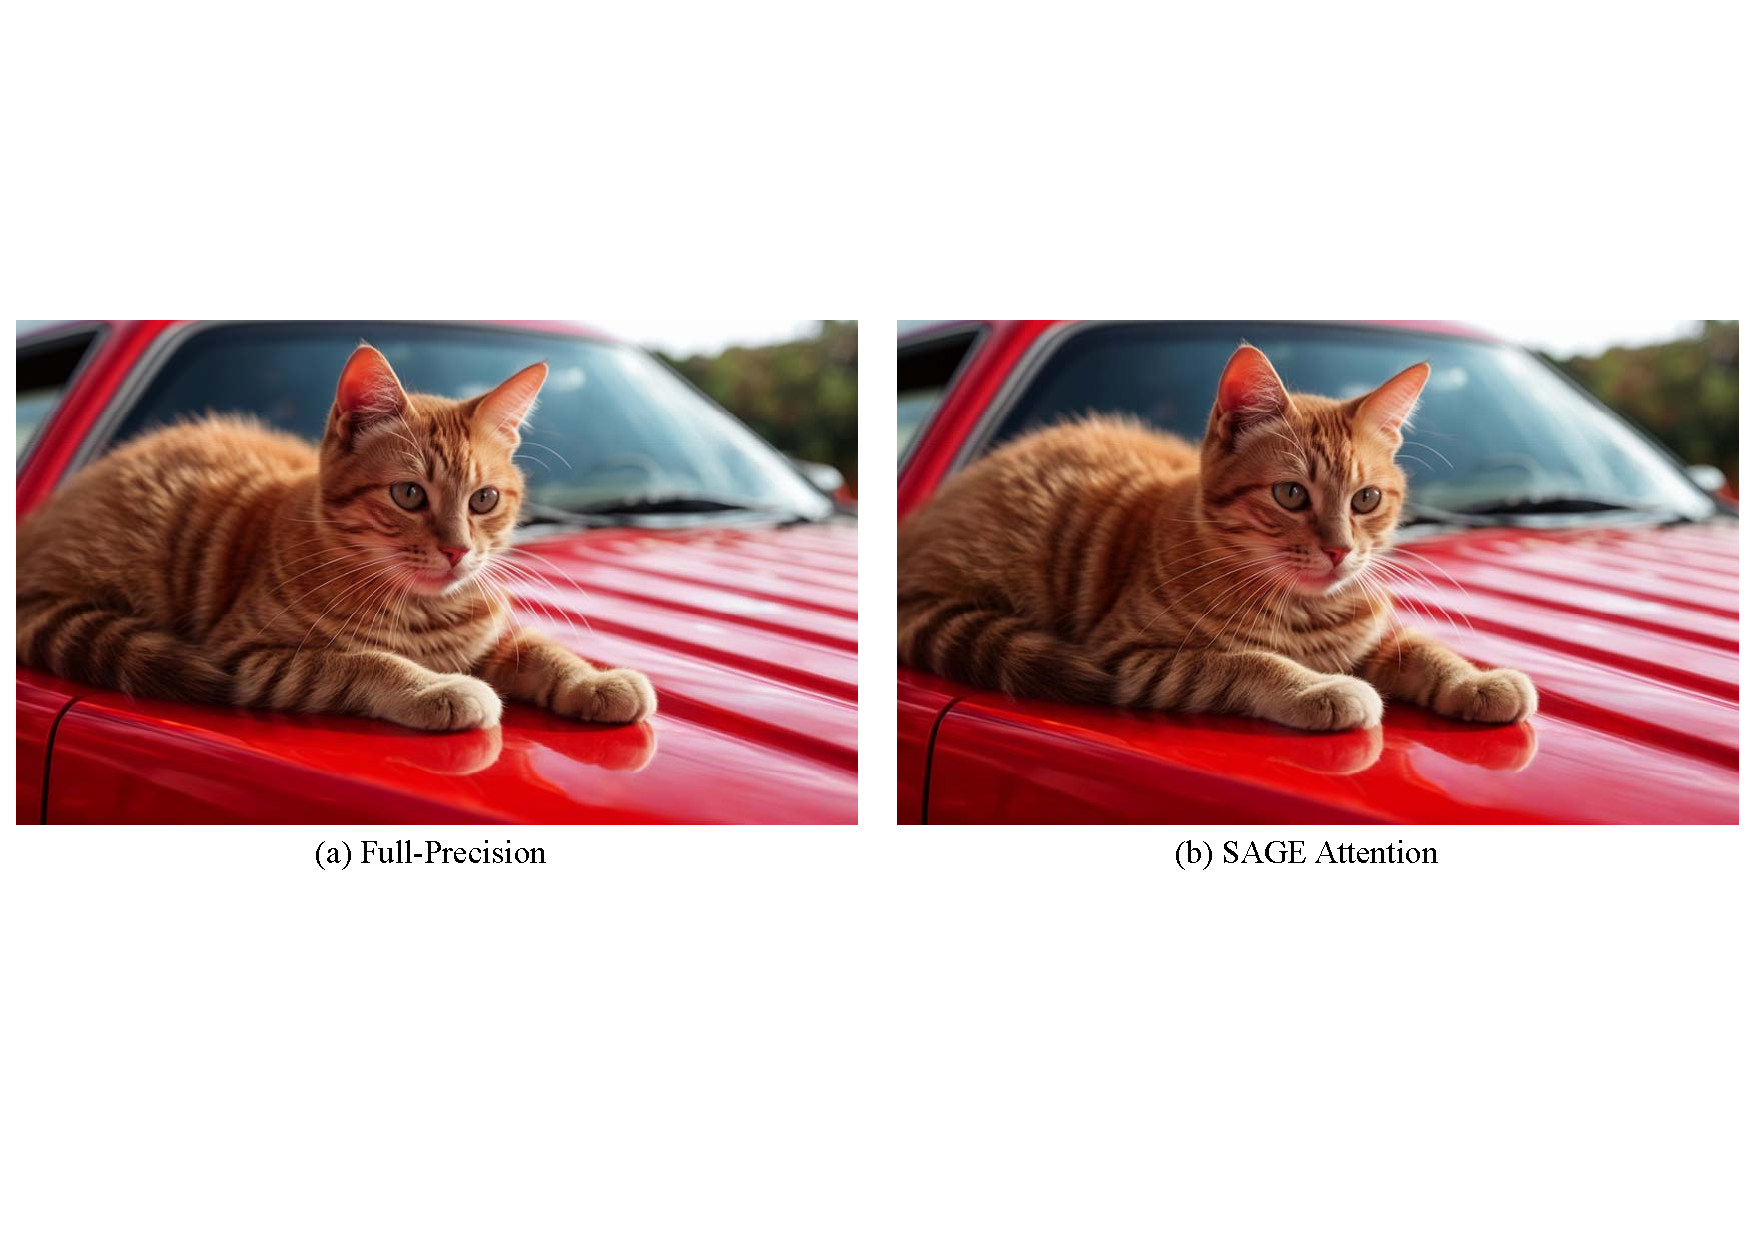
\includegraphics[width=.96\textwidth]{figs/ultrapixel.pdf}
    \caption{An image generation example of UltraPixel.}
    \label{fig:ultrapixel}
\end{figure}

\begin{figure}[!htb]
    \centering
    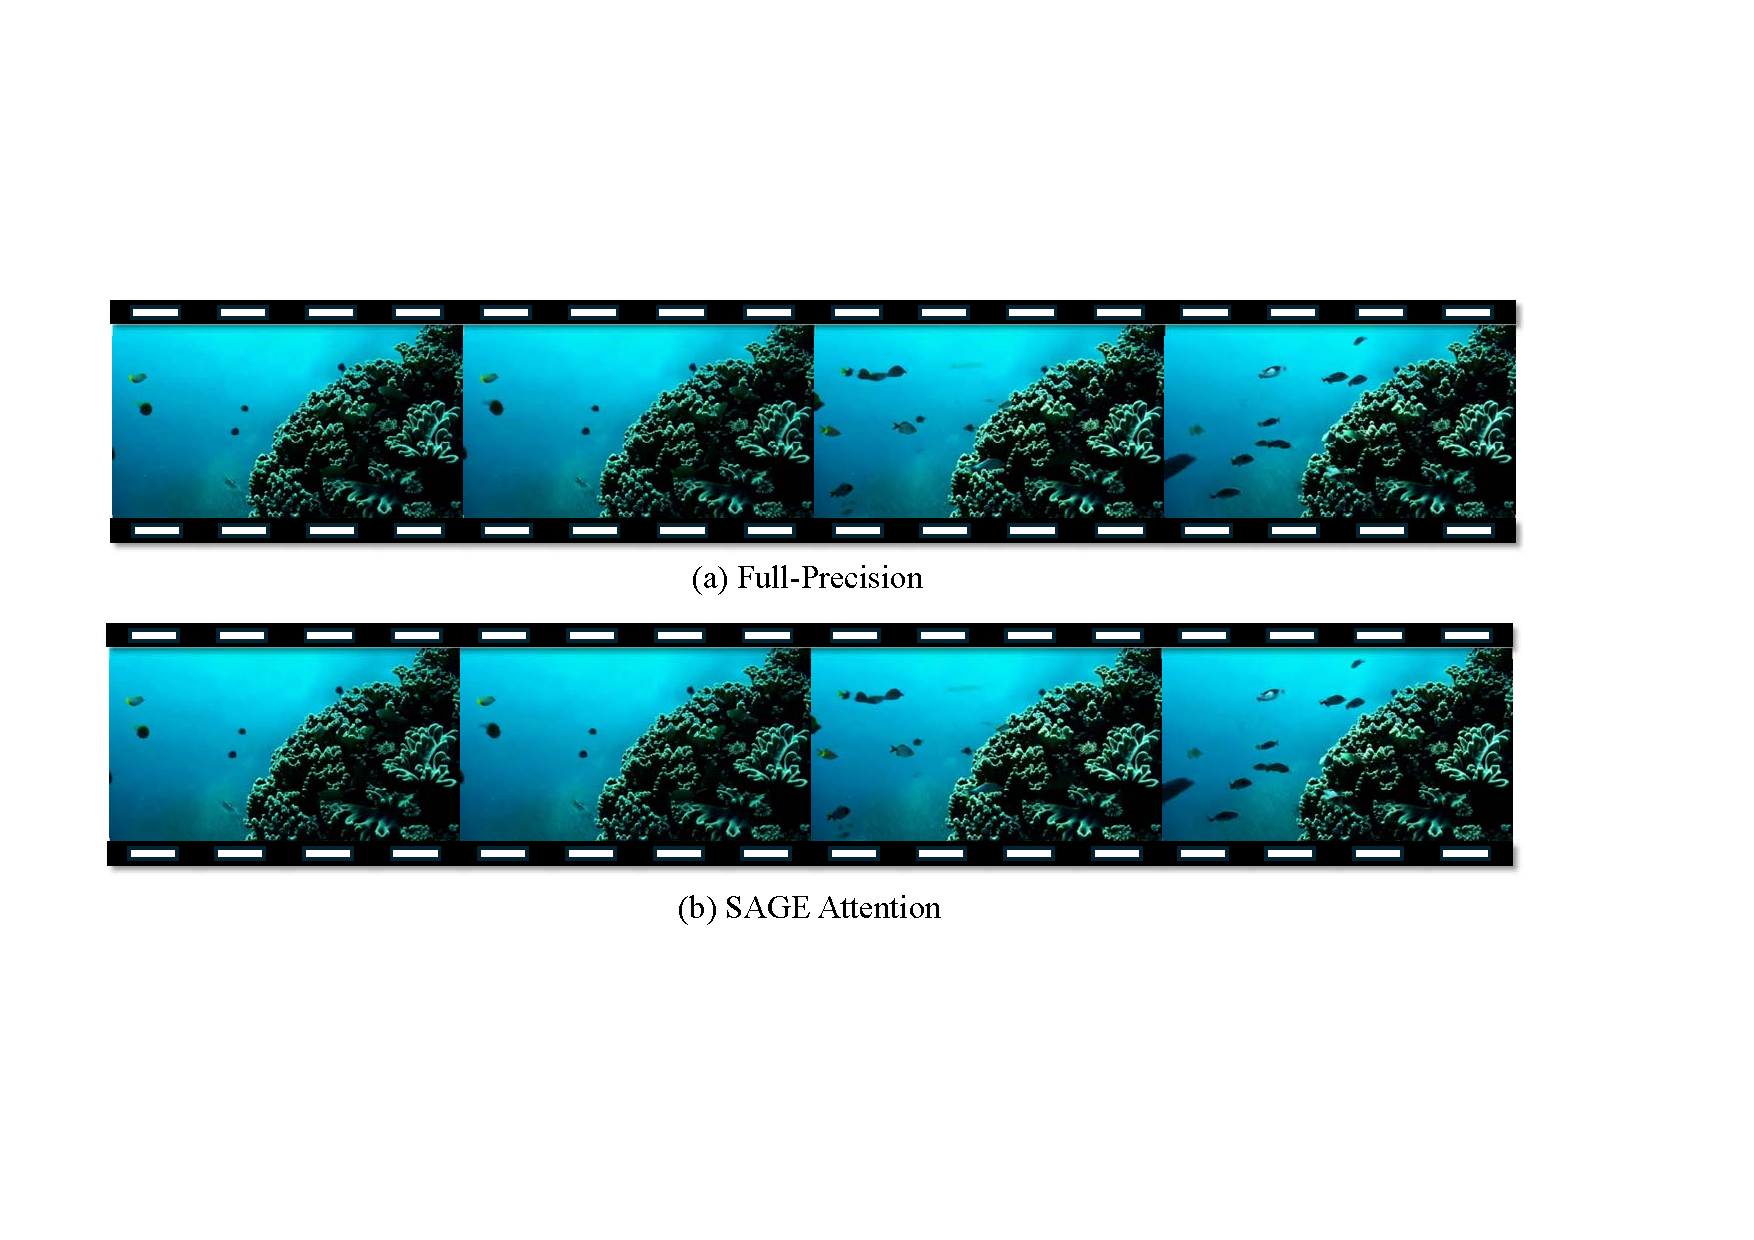
\includegraphics[width=.96\textwidth]{figs/Opensora.pdf}
    \caption{A video generation example of Open-Sora.}
    \label{fig:opensora}
\end{figure}

\begin{figure}[!htb]
    \centering
    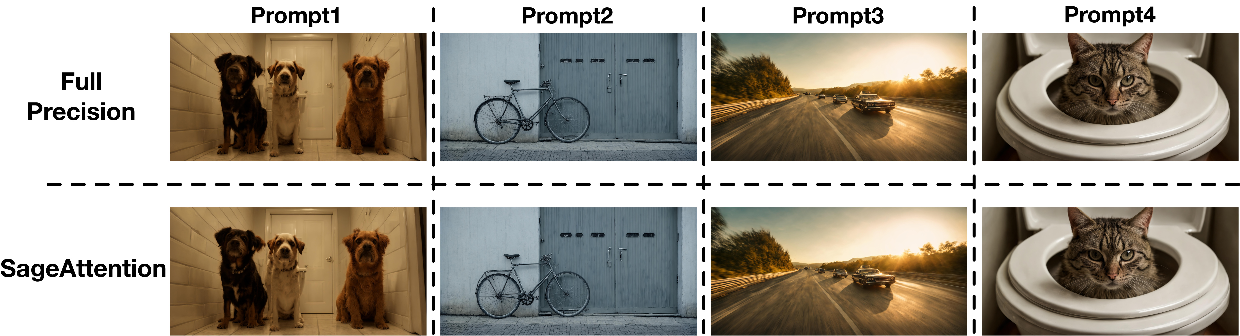
\includegraphics[width=.99\textwidth]{figs/rebuttal_image_video_tex.pdf}
    \caption{\purple{More image generation examples of UltraPixel, where prompt1="Two dogs are looking up while they stand near the toilet in the bathroom", prompt2="A gray bicycle is locked to some metal doors", prompt3="An image of a car driving on the highway", and prompt4="A cat on the lid of a toilet looking perturbed".}}
    \label{fig:rebuttal_image_video1}
\end{figure}

\begin{figure}[!htb]
    \centering
    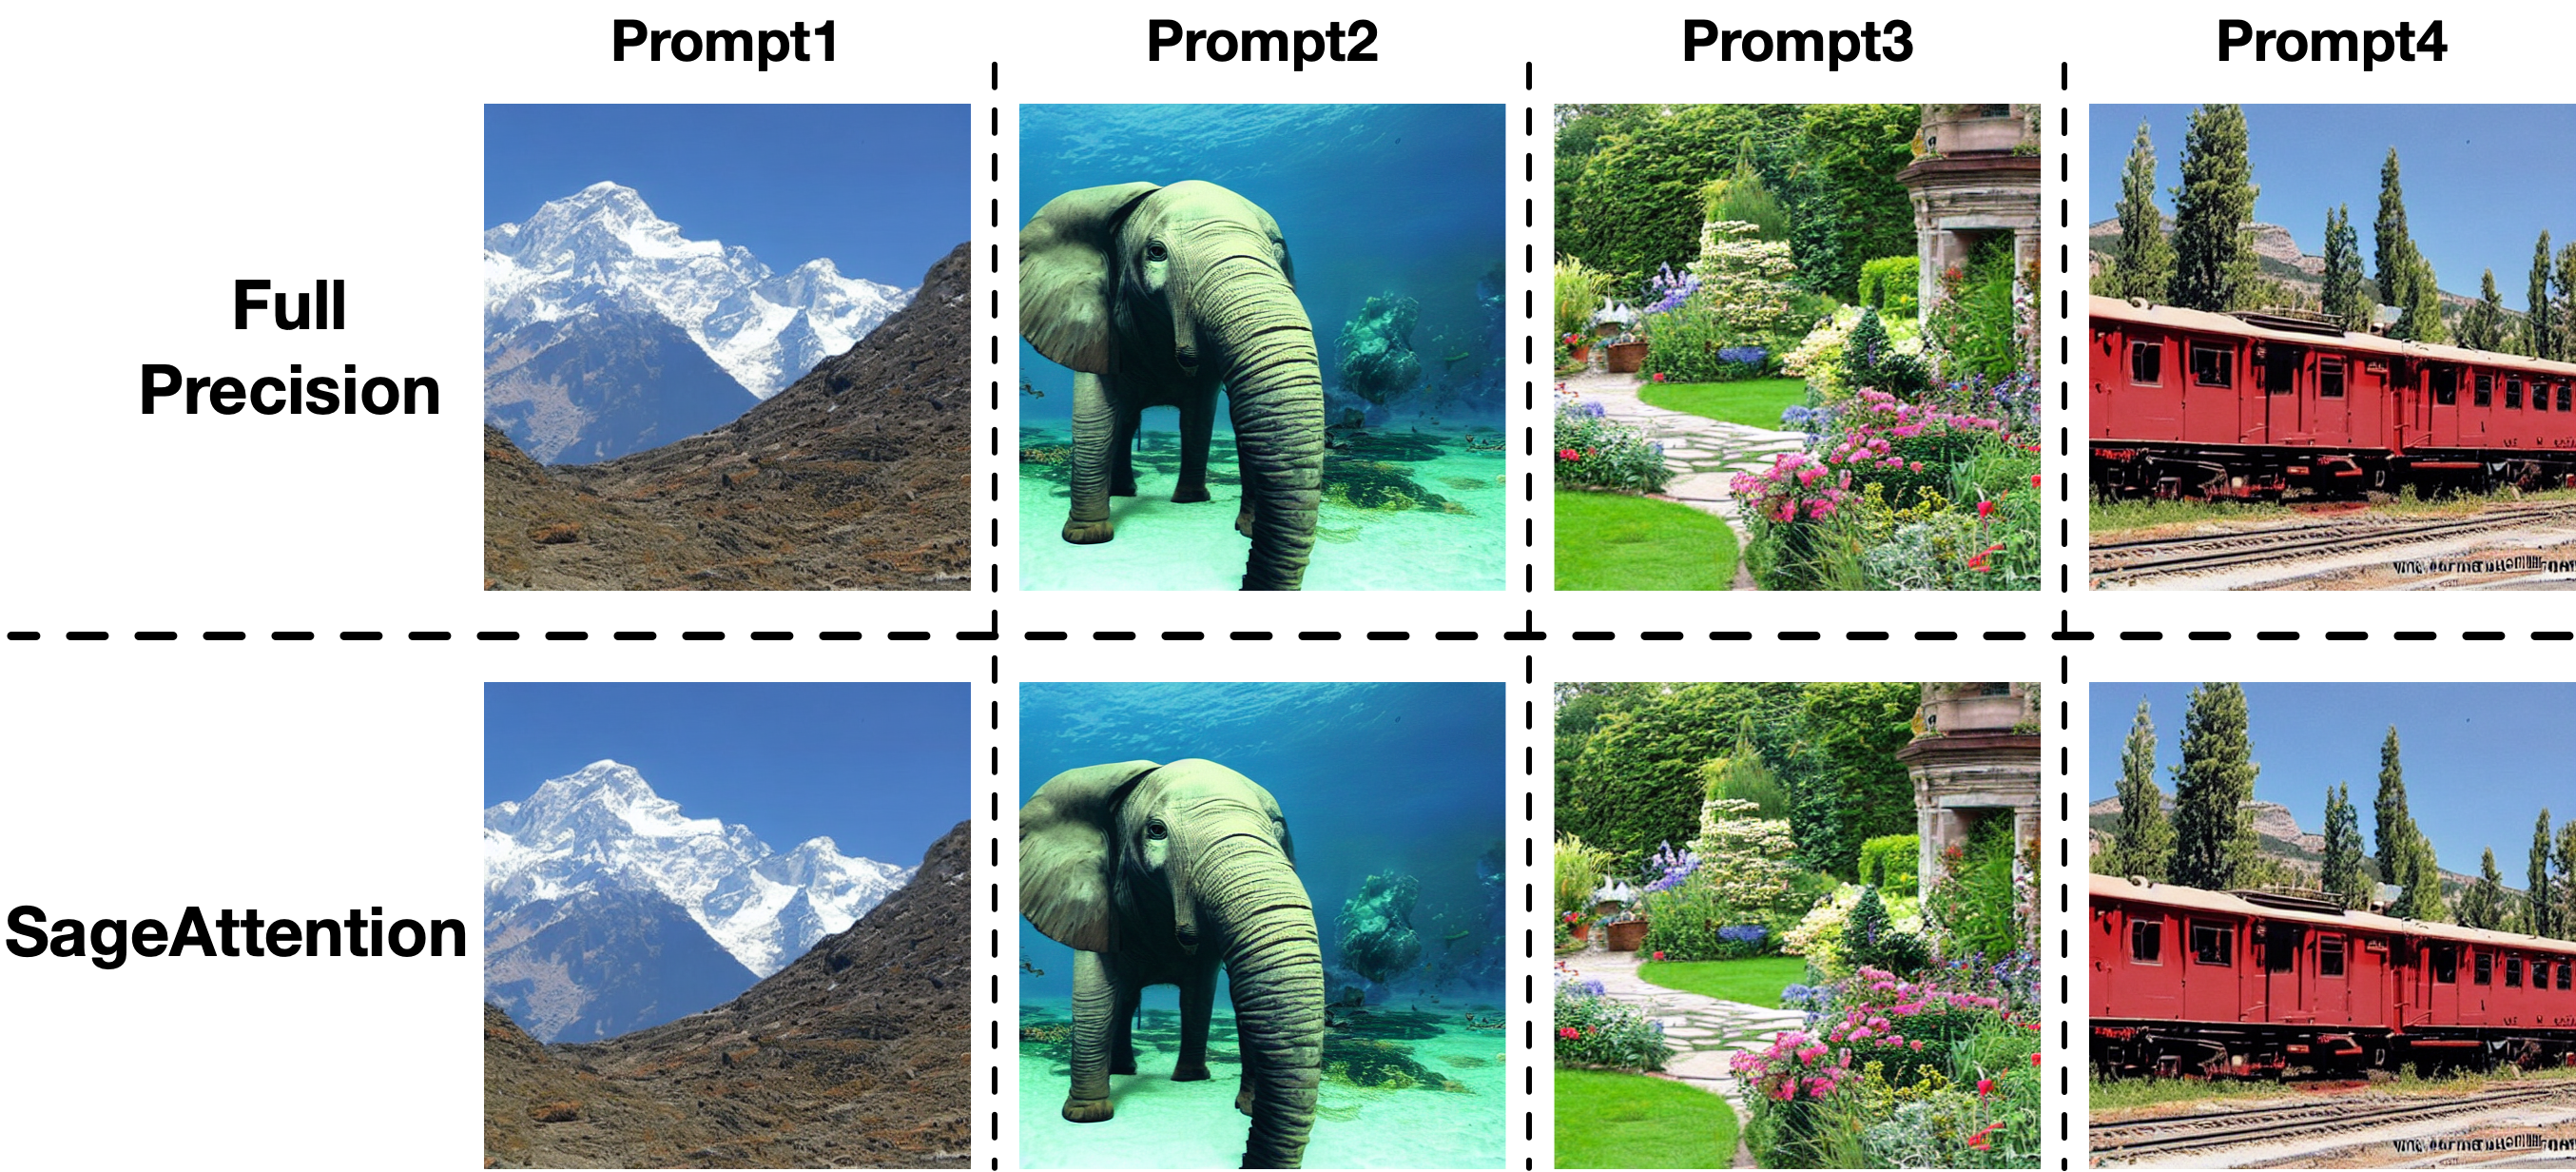
\includegraphics[width=.81\textwidth]{figs/rebuttal_image_video2.png}
    \caption{\purple{More image generation examples of Unidiffuser, where prompt1="Beautiful view of the Himalayas", prompt2="An elephant under the sea", prompt3="English Country Garden Design", and prompt4="An old red electric rail train in Durango, Colorado".}}
    \label{fig:rebuttal_image_video2}
\end{figure}

\begin{figure}[!htb]
    \centering
    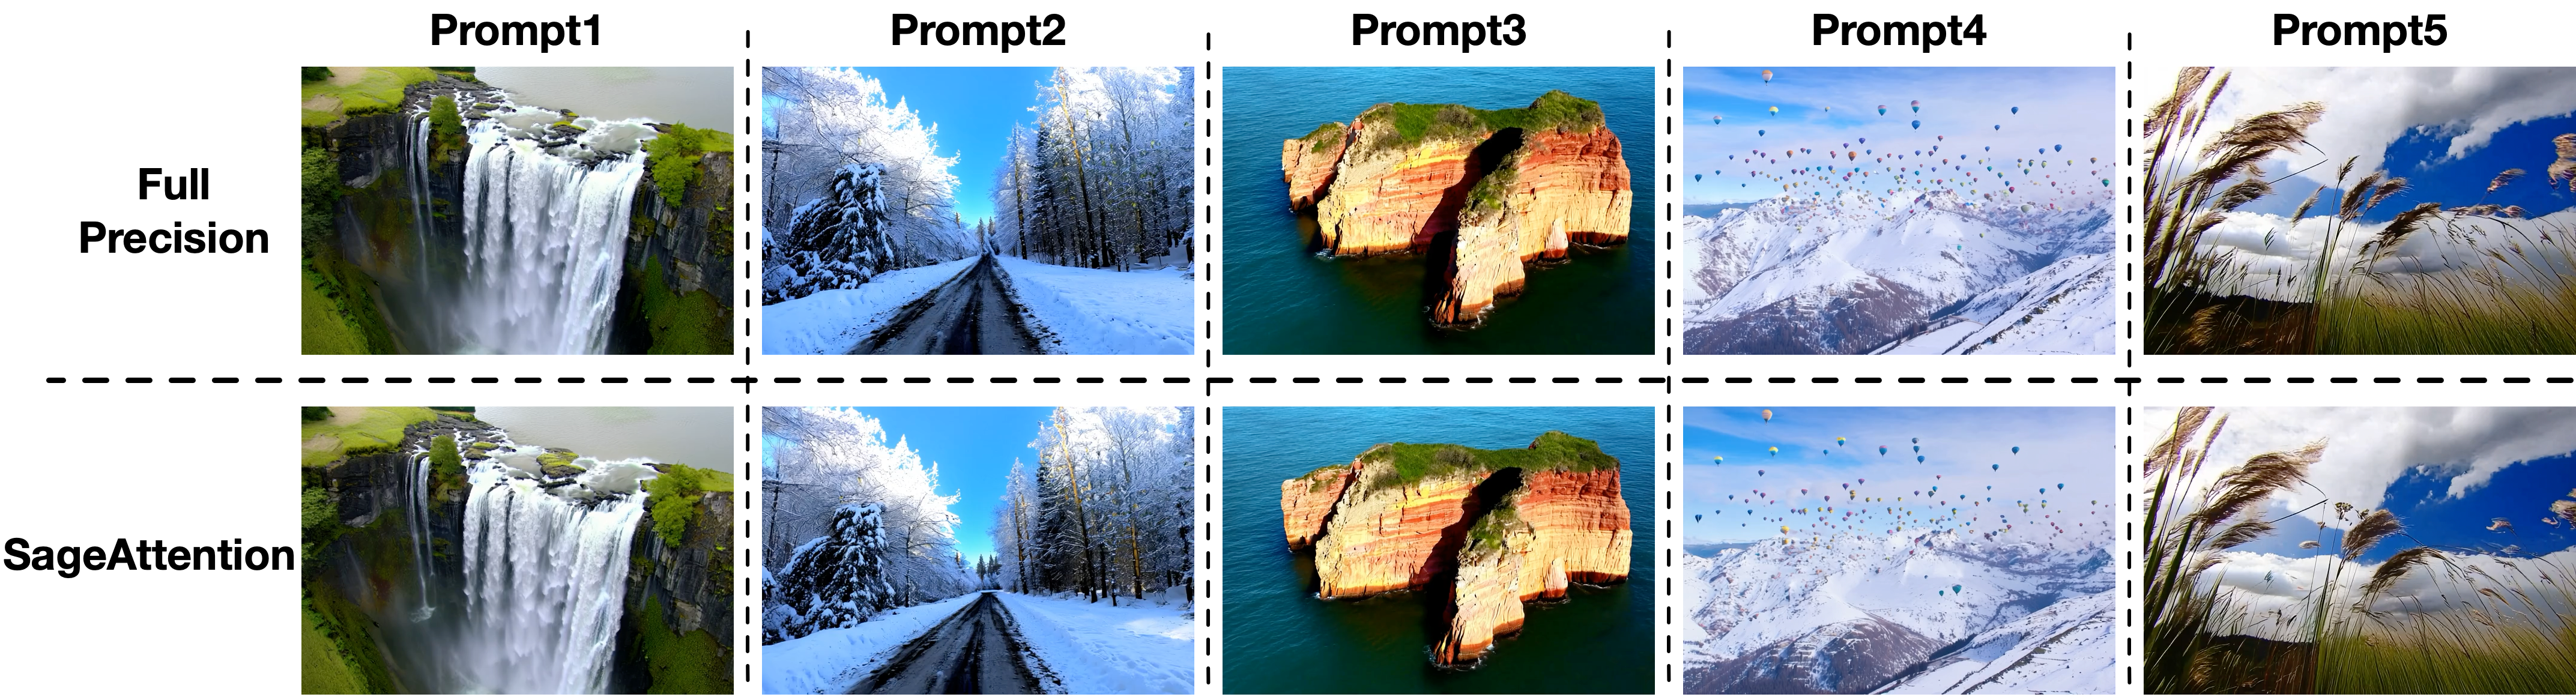
\includegraphics[width=.999\textwidth]{figs/rebuttal_image_video3.png}
    \caption{\purple{More image generation examples of CogvideoX. For more details about the prompts and the full videos, refer to \url{https://anonymous.4open.science/r/image_video_examples-3E44/README.md}.}
    \label{fig:rebuttal_image_video3}}
\end{figure}


\begin{table}[h!]
    \caption{Comparison of real speedup on RTX3090.}
    \label{exp:real_flops_3090}
    \begin{center}
    \begin{tabular}{l|c|l|c|c}
    \toprule
    {\bf Model}  & {\bf Shape of Q, K, V}  & {\bf Original Attention}  & {\bf SAGEAttention}  & {\bf Speedup}
    \\ \hline
    \cogvideo    & (2, 30, 17776, 64) &  71.57 (FlashAttn2)  &  \textbf{129.87}  & \cellcolor{gray!24}\textbf{1.81x}  \\
    \llama       & (4, 32, 1536, 128) &  56.54 (FlashAttn2)  &  \textbf{108.91}  & \cellcolor{gray!24}\textbf{1.93x}  \\ 
    \ultrapixel  & (2, 32, 7285, 64)  &  65.86 (FlashAttn2)  &  \textbf{131.74}  & \cellcolor{gray!24}\textbf{2.00x}  \\ 
    \unidiffuser & (4, 24, 1105, 64)  &  47.64 (xformers)    &  \textbf{108.91}  & \cellcolor{gray!24}\textbf{2.29x}  \\ 
    \timm        & (12, 64, 197, 64)  &  12.33 (Torch)        &  \textbf{66.34}  & \cellcolor{gray!24}\textbf{5.38x}  \\ \bottomrule
    \end{tabular}
    \end{center}
\end{table}



\subsection{Additional Precision Comparision}
Table~\ref{tab:qk_error} shows the precision of $Q \cdot K$ using per-token quantization in different data types compared to $Q \cdot K$ in full precision. This experiment is conducted using $Q, K$ from the 24th layer of \unidiffuser. It shows that quantizing $Q, K$ to INT8 performs higher precision than using E4M3 and E5M2.

Table~\ref{tab:append_smooth_k} shows the precision of different quantization methods with and without \textit{smoothing K} on various models. The results demonstrate that \textit{smoothing K} offers significant benefits of precision. 



\subsection{Visualized Results}
Figure~\ref{fig:ultrapixel} shows the high-resolution images (2560x1536) generated by \ultrapixel using Attention of full precision and \our.
It can be seen that \our matches the full precision in the high quality and highly detailed images.
Figure~\ref{fig:opensora} shows the videos (720x1280) generated by Open-Sora~\citep{opensora} in different precisions.
\our yields identically the same video as the full precision one.

\purple{Figure~\ref{fig:rebuttal_image_video1}, Figure~\ref{fig:rebuttal_image_video2}, and Figure~\ref{fig:rebuttal_image_video3} show more visualized comparison results on \ultrapixel, \unidiffuser, and \cogvideo.}


\subsection{Real Speedup on RTX3090}

We further measure the real speed of \our and the original Attention on \unidiffuser, \ultrapixel, \cogvideo, \llama and \timm on RTX3090. 
Table~\ref{exp:real_flops} shows that \our outperforms original attention across all models. Specifically, \our yields 2.7$\times$ speedup compared to the original Attentions on average.







